\section{Sistemi Monodimensionali}
    Definiamo il Sistema Monodimensionale: 
    \begin{figure}[H]
        \centering 
        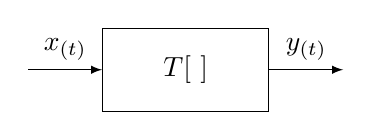
\begin{tikzpicture}[
            node distance=2cm,
            >=latex
            ]

            \node [coordinate] (input) {};
            \node [draw, rectangle,right of = input, minimum height=3em, minimum width=6em] (block) {$T[\ ]$};
            \node [coordinate, right of = block] (output) {};
            
            \draw[draw,->] (input) -- node[above]{$x_{(t)}$} (block);
            \draw[->] (block) -- node[above]{$y_{(t)}$} (output);
        \end{tikzpicture}    
    \label{Def sistema monodimensionale}
    \end{figure}
    Il sistema applica la trasformazione $T[\ ]: y_{(t)} = T[x_{(t)}]$ in gemerale \\ $y_{(t)} = T[x_{(\alpha)},t]$. 
    \subsection{Propietá dei Sistemi Lineari Tempo Invarianti (LTI)}
        \begin{itemize}
            \item {Linearitá:
                \[
                    x_{(t)} = ax_{1(t)}+bx_{2(t)} \overset{T[\ ]}{\Rightarrow} y_{(t)} = aT[x_{1(t)}]+b T[x_{2(t)}]
                \]
                Oppure separando la variabile del tempo:
                \[
                    x_{(t)} = ax_{1(t)}+bx_{2(t)} \overset{T[\ ]}{\Rightarrow} y_{(t)} = aT[x_{1(\alpha)},t]+b T[x_{2(\alpha)},t]
                \]
                É il principio di linearitá o sovrapposizione degli effetti visto a elettrotecnica.
            }\label{SM Linearita}
            \item {Stazionarietá:
                \[
                    y_{(t)} = T[x_{(t)}] \rightarrow y_{(t-t_0)} = T[x_{(t-t_0)}]  
                \]
            }\label{SM Stazionarieta}
            \item {Causalitá:
                \[
                    y_{(t)} = T[x_{(\alpha)},\alpha\leq t]
                \]
                L'uscita all'istante $t$ dipende dall'ingresso ad instanti precedenti o al piú uguali a $t$, si basa su valori precendenti a 
                $t$ non puó prevedere il futuro. Ne derivano 2 distinzioni di trasformazioni:
                \begin{itemize}
                    \item Real Time: necessariamente causale (é nel presente)
                    \item Virtual time: Causale o Non Causale (es. ho tutto un file al quale posso prevedere i bit o frame successivi per applicarne un post-processing)
                \end{itemize}
            }\label{SM Causalita}
            \item {Stabilitá BIBO:
                Se il segnale $x_{(t)}$ ha ampiezza limitata $\rightarrow$ l'uscita ha ampiezza limitata:
                    \[
                        |x_{(t)}|\leq M \rightarrow |y_{(t)}|\leq K 
                    \]
            }\label{SM Stabilita BIBO}
            \item {Invertibilitá:
                \[
                    y_{(t)} = T[x_{(\alpha)},t] \overset{\text{Se} \exists}{\Rightarrow} x_{(t)} = T^{-1}[y_{(\alpha)},t]
                \]
            }\label{SM Invertibilita}
            \item {Memoria:
                Un sistema é:
                \begin{itemize}
                    \item {Senza memoria: se $y_{(t)} = T[x_{(\alpha)},\alpha=t]$}
                    \item {Con Memoria: $y_{(t)} =\int_{-\infty}^{t}x_{(\alpha)} d\alpha$ l'uscita all'istante $t$ dipende anche da valori dell'ingresso 
                          ad istanti diversi da $t$. Nota bene é l'integrale di convoluzione di $x_{(t)} \otimes u_{(t)}$ 
                    }
                \end{itemize}
            }\label{SM Memoria}
        \end{itemize}
    \subsection{Propietá dei Sistemi Lineari Stazionari (SLS)}
        Sono sistemi che godono delle propietá di Linearitá \ref{SM Linearita} e di Stazionarietá \ref*{SM Stazionarieta}:
        \begin{figure}[H]
            \centering 
            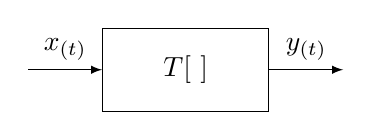
\begin{tikzpicture}[
                node distance=2cm,
                >=latex
                ]

                \node [coordinate] (input) {};
                \node [draw, rectangle,right of = input, minimum height=3em, minimum width=6em] (block) {$T[\ ]$};
                \node [coordinate, right of = block] (output) {};
                
                \draw[draw,->] (input) -- node[above]{$x_{(t)}$} (block);
                \draw[->] (block) -- node[above]{$y_{(t)}$} (output);
            \end{tikzpicture}    
        \label{Def SLS}
        \end{figure}  
        Troviamo la relazione tra ingresso e uscita:
        \begin{align}
            y_{(t)} &= T[x_{(\alpha)},t] =T[x_{(t)}] = T[x_{(t)} \otimes \delta_{(t)}] = T[\int_{-\infty}^{\infty}x_{(\alpha)}\delta_{(t-\alpha)}d\alpha]\nonumber \\        
                    &\overset{\ref*{SM Linearita}}{\Rightarrow} \underset{(\alpha)}{\int_{-\infty}^{\infty}}\underset{(t)}{T}[x_{(\alpha)}\delta_{(t-\alpha)}]d\alpha =\underset{(\alpha)}{\int_{-\infty}^{\infty}}x_{(\alpha)}\underset{(t)}{T}[\delta_{(t-\alpha)}]d\alpha\nonumber         
        \end{align}  
        Definiamo la trasformata nota del $\delta_{(t)}$:
        \begin{figure}[H]
            \centering 
            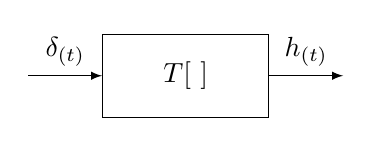
\begin{tikzpicture}[
                node distance=2cm,
                >=latex
                ]

                \node [coordinate] (input) {};
                \node [draw, rectangle,right of = input, minimum height=3em, minimum width=6em] (block) {$T[\ ]$};
                \node [coordinate, right of = block] (output) {};
                
                \draw[draw,->] (input) -- node[above]{$\delta_{(t)}$} (block);
                \draw[->] (block) -- node[above]{$h_{(t)}$} (output);
            \end{tikzpicture}    
        \label{Def impulso}
        \end{figure}
        Sollecitando il sistema con una Delta di Dirac ho la sua risposta impulsiva\index{Risposta Impulsiva}. Nel caso dei sistemi $SLS$ l'impulso
        in uscita caratterizza completamente il sistema. Nel nostro caso $T[\delta_{(t-\alpha)}]$ non é altro che una traslazione della $T[\delta_{(t)}]$ per la 
        Stazionarietá \ref*{SM Stazionarieta}: 
        \[
            y_{(t)} =\int_{-\infty}^{\infty}x_{(\alpha)}h_{(t-\alpha)}d\alpha = x_{(t)}\otimes h_{(t)} 
        \]
        La trasformata del sistema dipende solo dalla $h_{(t)}$. Passando al dominio della frequenza per la propietá della convoluzione \ref{Convoluzione}:
        \[
            y_{(t)} =X_{(f)}\otimes H_{(f)} 
        \]
        Dove$H_{(f)} = TCF[h_{(t)}] = \int_{-\infty}^{\infty} h_{(t)}e^{-j2\pi ft}$ é la risposta in frequenza del sistema $SLS$. Esistono vari modi
        per calcolare $h_{(t)}$:
        \begin{itemize}
            \item {
                
            }
        \end{itemize}
    \subsection{Risposta di un sistema causale e risposta impulsiva}
    